\documentclass[12pt]{article}
\usepackage{amsmath}
\usepackage{graphicx}
\usepackage{pdfpages}
\usepackage{amssymb}

\title{Exercise Set 8.5}
\author{Ryan C. Bleile}

\begin{document}
\maketitle

\newpage

\section*{Question 5 Resubmitted}

Investigate the critical point (1,1) of:

\[ f = 2 - 2x^{2} + 2x + 2y^{2} - 3y - xy + x^{3} \]

We will begin by using a quadratic approximation of our function around the critical point. This approximation can be computed in this manner:

\[ f(x,y) \approx f(1,1) +
\begin{bmatrix}
\frac{df}{dx}(1,1) & \frac{df}{dy}(1,1)
\end{bmatrix}
\begin{bmatrix}
x\\
y
\end{bmatrix}
+
\frac{1}{2}
\begin{bmatrix}
x & y
\end{bmatrix}
\begin{bmatrix}
\frac{d^{2}f}{dx^{2}}(1,1) & \frac{d^{2}f}{dxdy}(1,1)\\
\frac{d^{2}f}{dydx}(1,1) & \frac{d^{2}f}{dy^{2}}(1,1)
\end{bmatrix}
\begin{bmatrix}
x\\
y
\end{bmatrix}
\]

So now taking all of the partial derivatives:

\begin{eqnarray}
f(1,1) &=& 1\\
\frac{df}{dx}(1,1)&=& 2\\
\frac{df}{dy}(1,1)&=& 0\\
\frac{d^{2}f}{dx^{2}}(1,1) &=& 2\\
\frac{d^{2}f}{dxdy}(1,1) &=& \frac{d^{2}f}{dydx}(1,1)\\
\frac{d^{2}f}{dydx}(1,1) &=& -1\\
\frac{d^{2}f}{dy^{2}}(1,1) &=& 4
\end{eqnarray}

This gives us:

\[
f(x,y) \approx 1 + 
\begin{bmatrix}
2 & 0
\end{bmatrix}
\begin{bmatrix}
x\\
y
\end{bmatrix}
+
\frac{1}{2}
\begin{bmatrix}
x & y
\end{bmatrix}
\begin{bmatrix}
2 & -1\\
-1 & 4
\end{bmatrix}
\begin{bmatrix}
x\\
y
\end{bmatrix}
\]

so using the methods of quadratic approximation we will take the expression: f(x,y) - f(1,1) and use this to approximate the function around the critical point. We will use a close inspection of the quadratic term in the approximation, whose matrix is refereed to as the Hessian, in order to gain an understanding of the area around the point (1,1). So taking the quadratic term lets call the vector <x,y> by $\vec{X}$ and the Hessian matrix H. The goal is now to determine if the product of the quadratic section denoted by $\vec{X}^{T}H\vec{X}$ is positive, negative or zero. Positive and we have a minimum. Negative and we have a maximum. Zero and we have not enough information to proceed and we must continue on to higher order approximations.\\

In order to see if  $\vec{X}^{T}H\vec{X}$ is positive, negative or zero it is helpful to use eigenvalue decomposition of H. And Since H is a symmetric we are guaranteed to have real eigenvectors, which can be scaled such that our eigenvectors are of unit length. this will give us that the eigenvector matrix V has an inverse $V^{-1}$ equal to its transpose $V^{T}$. Using this and eigenvalue decomposition we get:

\begin{eqnarray}
\frac{1}{2} \vec{X}^{T}H\vec{X}\\
\frac{1}{2} \vec{X}^{T}(V \Lambda V^{T})\vec{X}\\
\frac{1}{2} (V^{T}\vec{X})^{T} \Lambda (V^{T}\vec{X})\\
V^{T}\vec{X} = \omega\\
\frac{1}{2} \omega^{T} \Lambda \omega\\
\frac{1}{2}( \lambda_{1} \omega_{1}^{2} + \lambda_{2} \omega_{2}^{2} )
\end{eqnarray}

We have just found an expression that contains all the required information. All that is left is to solve for $\omega$ and the eigenvalues $\lambda_1$ and $\lambda_2$

\[
[V,D] = eig(H)
\]
Yeilds:
\[
D = 
\begin{bmatrix}
3-\sqrt{2} & 0\\
0 & 3 + \sqrt{2}
\end{bmatrix}
or\ 
\begin{bmatrix}
1.5858 & 0\\
0 & 4.4142
\end{bmatrix}
\]
\[
V = 
\begin{bmatrix}
 -0.9239 &  -0.3827\\
   -0.3827  &  0.9239
\end{bmatrix}
\]

which can be put together to give us the result:

\[
V^{T}\vec{X} = 
\begin{bmatrix}
 -1.3066\\
    0.5412
\end{bmatrix}
\]

which we can now use to fill in our equation and see that:

\begin{eqnarray}
\frac{1}{2}( \lambda_{1} \omega_{1}^{2} + \lambda_{2} \omega_{2}^{2} )\\
\frac{1}{2}(1.5858*-1.3066 + 4.4142*.5412 )\\
.1579
\end{eqnarray}

is positive. And there for the critical point is a minimum. In order to provide further proof here is a plot of the minimum around the inflection point.

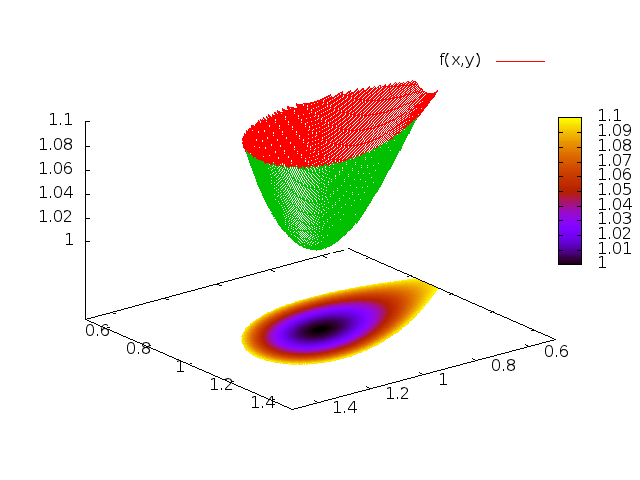
\includegraphics[scale=.5]{Minplot.png}\\
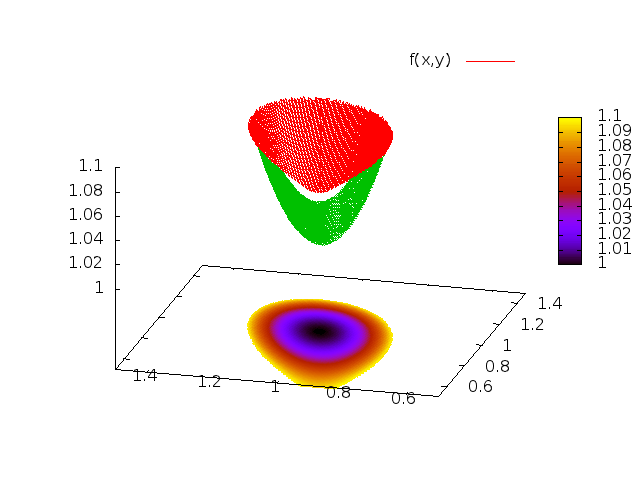
\includegraphics[scale=.5]{Minplot2.png}

\end{document}
